\documentclass[12pt]{article}
% General packages
\usepackage{amsmath, graphicx, float, tabularx, booktabs, color}
% For adjusting margin size
\usepackage[margin=1in]{geometry}
% For setting bookmarks on pdf export
\usepackage[bookmarks,bookmarksopen,bookmarksdepth=2]{hyperref}
% For codeblocks
\usepackage{listings}
\usepackage{cite}

%Define Colors
\definecolor{dkgreen}{rgb}{0,0.6,0}
\definecolor{gray}{rgb}{0.5,0.5,0.5}
\definecolor{mauve}{rgb}{0.58,0,0.82}

% Color Code
\lstset{frame=tb,
  language=ruby,
  aboveskip=3mm,
  belowskip=3mm,
  showstringspaces=false,
  columns=flexible,
  basicstyle={\small\ttfamily},
  numbers=none,
  numberstyle=\tiny\color{gray},
  keywordstyle=\color{blue},
  commentstyle=\color{dkgreen},
  stringstyle=\color{mauve},
  breaklines=true,
  breakatwhitespace=true,
  tabsize=4
}

% Image path location
\graphicspath{ {images/} }

\begin{document}

% Title information
\title{Buffer Overflow SLMail-5.5.0 Service and Gain Root Shell}
\author{Devin Trejo \tabularnewline devin.trejo@temple.edu}
\date{\today}
\maketitle

\section{Summary}
\label{sect:summary}


\section{Introduction}
\label{sect:intro}
\subsection{Background SLMail5.5.0}
\label{sec:background}
SLMail is a message management tool that was advertised towards small to 
medium sized businesses published by SeatleLabs. The software was popular 
around the year 2001 for its ease of use and ``security'' of its email 
service \cite{SeattleLabs2001}. The service was also scalable for an 
unlimited number of users to use. The software boast a number of security 
features including, ``Limiting viruses by identifying specific files or types 
not permitted to enter/leave the server, rejecting emails containing unwanted 
words, avoiding external use of server as relay for spam, reduce flow of 
junk mail (anti-spam filter), and authenticate users before they send 
mail'' \cite{SeattleLabs2001}. The last ``security'' feature was instead a 
security flaw as the password authentication had a buffer overflow 
vulnerability. The service is no longer developed as is apparent if one
were to search for SLMail on SeattleLabs' website today. 

The SLMail service is an 3rd party program bought and downloaded direct
from SeattleLabs's website and typically installed on a Windows 2k server.
The default options after a succesfull installation of SLMail
can be seen in figure~\ref{fig:deafconfigslmail}. The specific version we 
concern ourselves for this project will by \textbf{SLMail5.5.0} which has a 
known buffer overflow exploit inside the user authentication prompt. When 
logging in over POP3, an application standard protocol for retrieving 
emails from a remote server, SLMail will prompt for a user-name and 
password combination associated with the desired email. If we write our 
user-name as any string combination and a password containing a shell program 
we can setup and execute the script on the remote mail server. The referenced 
shell script will be specially crafted to open a port on the remote server, 
that gives us access to a shell that contains administrative privileges. 

\begin{figure}[ht]
    \centering
    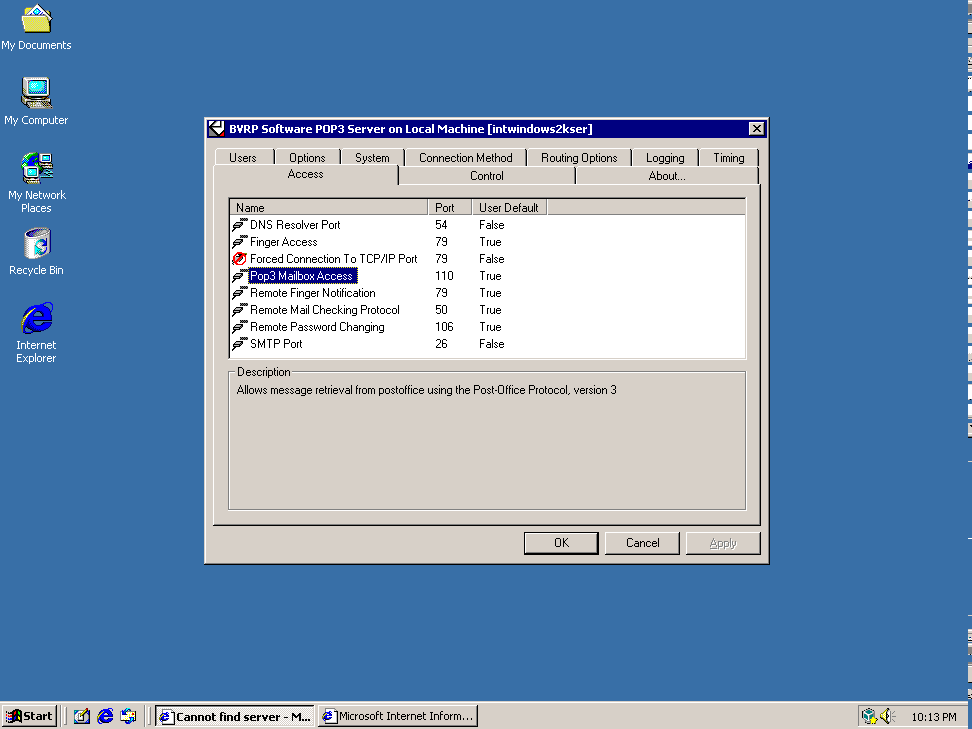
\includegraphics[width=5.5in]{images/20160407_slmail_config.png}
    \caption{Default SLMAail Port Configuration}
    \label{fig:deafconfigslmail}
\end{figure}

\subsection{Attack Approach: Fuzzing Attack}
\label{sec:approachpassbuff}

The first step for this attack is to gain more information of the
SLMail 5.5.0 service. We will implement a technique known as \textbf{fuzzing}
which will allow us to discover information such as service versions, 
buffer sizes, and in general the coding implementation of the remote
service. To begin the fuzzing process, we try to find the buffer size of the 
PASS field used by SLMail's POP3 protocol. The first step is to write a 
script that loops over an array of increasing buffer sizes trying to 
determine the full length of the input buffer size. Since we already know 
there is an buffer overflow exploit for these fields we can expect at some 
point our input to overflow the allocated buffer and crash the program. 
The idea and goal for this specific fuzzing processes is to overwrite the 
\textbf{EIP register} or the address location on the program stack 
containing the location in memory the program should return to after 
executing the USER and PASS input prompt function.

For this assignment we will examine the structure of the SLMail-5.5.0 
program and gain insights on its construction. The POP3 interface seen on 
port 101 is not compatible with standard the standard http protocol as is 
demonstrated in figure~\ref{fig:smailpop3http}. Instead we write a Python
script that creates a socket connection to the POP3 service and interfaces
with the server using POP3 protocol commands. 

\begin{figure}[ht]
    \centering
    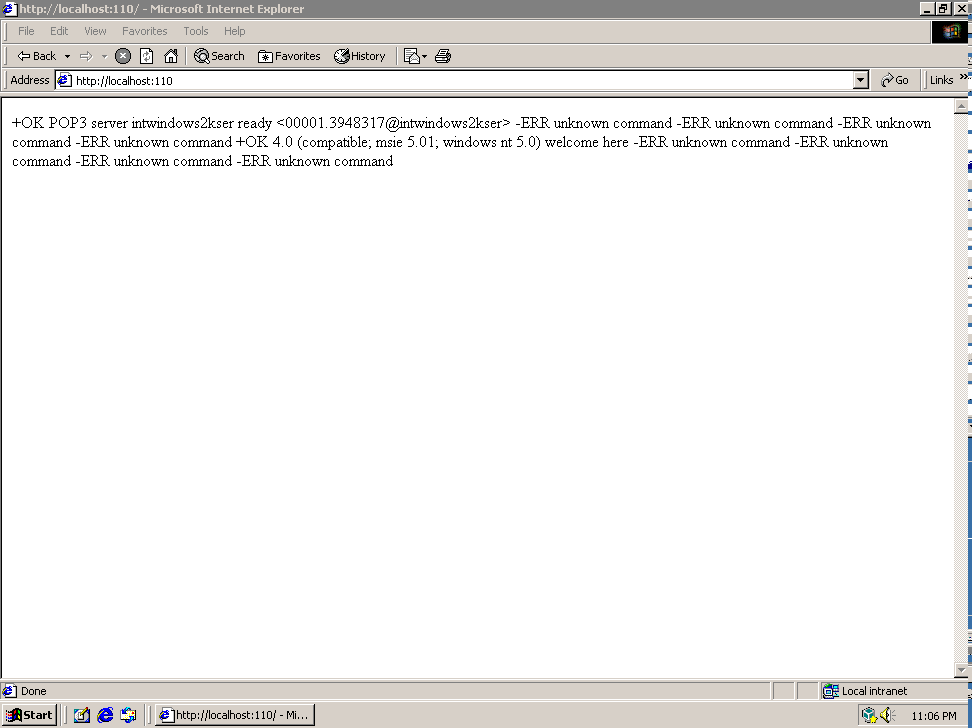
\includegraphics[width=5.5in]{images/20160407_http_smail.png}
    \caption{Trying to Connect to SLMail POP3 over HTTP}
    \label{fig:smailpop3http}
\end{figure}

\subsection{Test Environment}
\label{sec:testenv}
For this project we use our default test environment. We have a virtual 
private network consisting of our Windows 2000 SP4 Server, Kali Linux
penetrating machine, and a host machine running through Oracle Virtual Box. 
The virtual network has a DHCP server running on the VM host machine. The 
IP/MAC addresses for each are provided in table~\ref{table:pentestnetwork}.

\begin{table}[H]
    \centering
    \begin{tabularx}{\textwidth}{|*{3}{>{\centering}X|}}
        \toprule
        \textbf{Platform} & \textbf{MAC ADDR} & \textbf{Platform IPv4 Address} 
        \tabularnewline \midrule
        \textbf{Kali Linux:} & 08:00:27:94:5b:ba & 192.168.56.102 
        \tabularnewline
        \textbf{Windows 2k Server:} & 08:00:27:87:29:68 & 192.168.56.105
        \tabularnewline
        \textbf{VM Host Machine:} & 08:00:27:7c:86:0d & 192.168.56.100
        \tabularnewline \bottomrule
    \end{tabularx}
    \caption{IP Configuration for SLMail Pen-test Virtual Network}
    \label{table:pentestnetwork}
\end{table}

\section{Discussion}
\label{sect:discussion}
To begin the intrusion we first have to setup our SLMail server. For this
test we used default parameters as seen in figure~\ref{fig:deafconfigslmail}.
Next we conducted a NMAP scan from our Kali Linux Machine using NMAP. The
scan we performed was a full version scan using the parameters seen shown 
below.

\begin{lstlisting}[language=bash]
    $ nmap -nsV 192.168.56.105
\end{lstlisting}

\begin{figure}[ht]
    \centering
    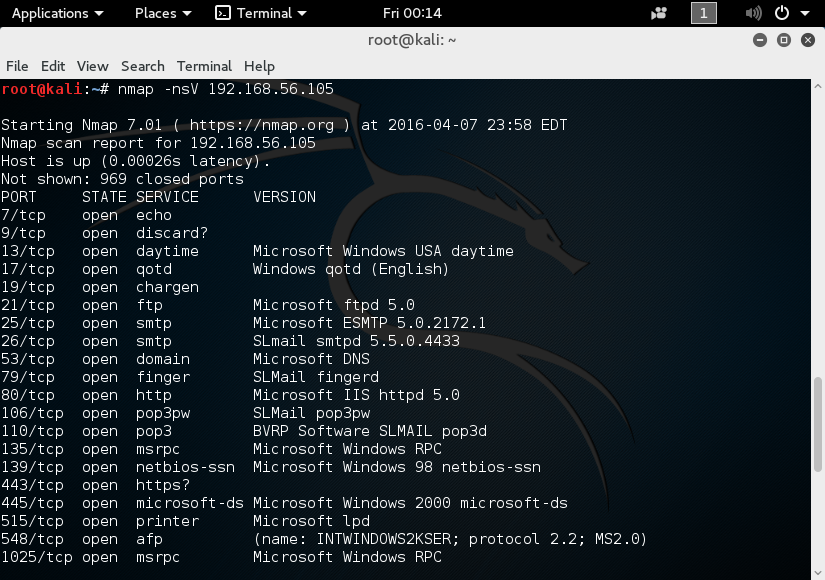
\includegraphics[width=5.5in]{images/20160407_nmap_scan.png}
    \caption{NMAP Scan of Windows Server 2k}
    \label{fig:nmapwindows}
\end{figure}

From the scan results seen in figure~\ref{fig:nmapwindows} we can see a
multitude of open ports and the services running behind the ports. What we are
interested in is port 110 which is the standard port for POP3 operations. We
know from our research that after installing SLMail an open POP3 port will
open that contains the known buffer overflow vulnerability. The NMAP scan 
revealed a number of other services running on our Windows 2k Server instance 
but for this test we will focus on port 110. 


\section{Conclusion}
\label{sect:conclusion}


\nocite{*}
\bibliographystyle{IEEEtran}
\bibliography{./20160407_project.bib}

\section*{Appendix}
\label{sect:appendix}
\lstinputlisting[language=Python, 
caption=SLMail Password Fuzzing Script,
label=lst:passFuzz]{slmail_buffer_overflow.py}

\end{document}